\subsection{Automatyczne kolorowanie czarno-białych obrazów}

  Problem kolorowania czarno-białych obrazów cieszy się dużym zainteresowaniem z
  wielu powodów. Od potrzeb kulturowych takich jak możliwość lepszego
  zwizualizowania oraz zrozumienia przeszłości poprzez kolorowania zdjęć z
  czasów, kiedy występowały one jedynie w kolorach czerni i bieli, po potrzeby
  technologiczne takie jak rekonstrukcja filmów oraz poprawa obrazu cyfrowego.

  Pomimo braku informacji o kolorze w czarno-białych zdjęciach, ludzie są w
  stanie określić potencjalne, rzeczywiste barwy obiektów na zdjęciach bazując
  na treści tych zdjęć oraz swoim doświadczeniu. Można z tego wywnioskować, że
  zdjęcia te zawierają informacje wystarczające do oszacowania potencjalnych
  kolorów. Pozwala to założyć, że do tego zagadnienia można skutecznie wykorzystać
  konwolucyjne sieci neuronowe, które cechują się niezwykłą umiejętnością do
  rozpoznawania wzorców oraz posiadają wyjątkowe zdolności do adaptacji. Z tego
  właśnie powodu sieci splotowe zostaną użyte w przedstawionym rozwiązaniu.

  \subsubsection{Podejście}

  Rozważając możliwe sposoby pokolorowania czarno-białego zdjęcia można spostrzec,
  że kiedy niektóre powierzchnie na zdjęciu mają zazwyczaj oczywiste barwy, niebo
  jest zazwyczaj niebieskie, a trawa zielona, to są też powierzchnie, które
  posiadają szeroki wachlarz możliwych kolorów, na przykład samochodów może być
  zarówno czerwony jak i niebieski albo zielony. Z tego powodu celem zaprezentowanego
  rozwiązania jest niekoniecznie odtworzenie rzeczywistych barw obrazu, a raczej
  wygenerowanie barw, które mogłyby być barwami rzeczywistymi.

  Aby zwiększyć efektywność uczenia wykorzystano przestrzeń barw CIELab. W tej
  przestrzeni barwę obrazu opisują 3 składowe:
  \begin{itemize}
  \item L -jasność (luminacja)
  \item A -barwa od zielonej do magenty
  \item B - barwa od niebieskiej do żółtej
  \end{itemize}
  Przestrzeń barw CIELab została przedstawiona na Rysunku \ref{fig:CIELab}

  \begin{figure}[ht]
    \centering
    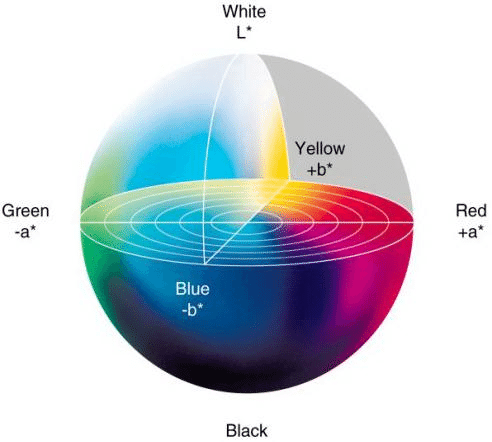
\includegraphics[width=4in]{CIELab}
    \caption[Przestrzeń barw CIELab - źródło:
    \url{https://www.flickr.com/photos/greenmambagreenmamba/4236391637}]
    {Przestrzeń barw CIELab.}
    \label{fig:CIELab}
  \end{figure}

  Zaletą zastosowania CIELab jest fakt, że jest ona najbardziej równomierną
  przestrzenią barw, co oznacza, że jeśli barwy znajdują się w jednakowej
  odległości od siebie w tej przestrzeni, to będą one postrzegane jako jednakowo
  różniące się od siebie. Powinno to zwiększyć skuteczność uczenia sieci oraz
  zapewnić bardziej realistyczne kolorowanie.

  Składowa \textit{L}, jako, że jest identyczna dla obrazu kolorowego jak i
  czarno-białego, stanowi w tym przypadku wejście sieci, na jej podstawie sieć
  odtwarza składowe \textit{A} oraz \textit{B}, które reprezentują przewidziane
  kolory dla obrazu wejściowego.

  Jako rozwiązanie podanej problematyki wpierw został oceniony autorski
  model podstawowy, na jego podstawie zostało przeprowadzone porównanie skuteczności
  różnych konfiguracji, w których uczony był model. Do elementów poddanych
  testom należą algorytm optymalizacyjny, funkcja straty, funkcja aktywacja oraz
  sposób przetwarzania wstępnego danych treningowych.

  \subsubsection{Model podstawowy}

  Opracowany przez nas model jest to FCN. Konwolucyjna część sieci składa się
  z 12 warstw splotowych
  mających na celu nauczyć się mapować składową wejściową \textit{L} na wyjściowe
  składowe \textit{A} i \textit{B}. Składowe wyjściowe muszą mieć takie same
  wymiary jak składowa wejściowe, co oznacza, że kluczowym było odpowiednie dobranie
  parametrów warstw takich jak \textit{padding} (pol. otoczka), \textit{stride}
  (pol. krok) oraz wielkość filtrów. Architektura sieci została przedstawiona w
  tabeli \ref{table:model_architecture}.

  \begin{table}[h!]
  \centering
    \begin{tabular}{||c c c c||}
     \hline
     Col1 & Col2 & Col2 & Col3 \\ [0.5ex]
       \hline\hline
       1 & 6 & 87837 & 787 \\
       2 & 7 & 78 & 5415 \\
       3 & 545 & 778 & 7507 \\
       4 & 545 & 18744 & 7560 \\
       5 & 88 & 788 & 6344 \\ [1ex]
       \hline
    \end{tabular}
    \caption{Architektura modelu podstawowego.}
    \label{table:model_architecture}
  \end{table}

  Pierwsza warstwa konwolucyjna rozkłada wejściowy kanał na 32 kanały, co
  pozwala wyciągnąć z niego jak najwięcej informacji o cechach obrazu. Warstwa
  ta ma wielkość filtra 3x3, tak więc aby zachować wymiar kanałów zostały
  zastosowane parametry $\textit{padding}=1$ oraz $\textit{stride}=1$.

  Kolejne trzy warstwy ekstraktują z wejściowych 32 kanałów najbardziej istotne
  cechy związane z powiązaniem treści obrazu z szacowanym kolorem jego powierzchni.
  Warstwy te na swoje wyjście przekazują po 32 kanały zawierające wykryte
  powiązanie pomiędzy pikselami kanałów wejściowych.

  Warstwa piąta rozciąga wejściowe 32 kanały na 64 kanały, dzięki temu kolejne
  2 warstwy przyjmujące na wejście te 64 kanały i przekazujące je na wyjście są
  w stanie wydobyć z obrazu cechy o większym poziomie abstrakcji, co znacznie
  zwiększa skuteczność działania sieci.

  Warstwa ósma ogranicza ilość kanałów w sieci z 64 do 32 wyciągając z nich
  cechy najbardziej przydatne do rozwiązania danej problematyki. Kanały te są
  następnie ponownie przetwarzane przez warwę z wielkością filtru 3x3, co ma
  służyć agregacji rozłożonych cech w bardziej spójną całość, która może być
  już składana w pożądane wyjście.

  Kolejne dwie warstwy w sieci są to warstwy konwolucyjne o wielkości filtru 1x1,
  odpowiadają one warstwom gęstym i mają na celu przekonwertowanie wartości
  funkcji aktywacji z poprzednich warstw na wartości kolorów odpowiadających
  pikseli w przestrzeni barw CIELab. Ostatnia warstwa, również z filtrem o
  wielkości 1x1 zwija 32 kanały otrzymywane na wejściu do 2 kanałów odpowiadających
  składowym \textit{A} oraz \textit{B}, które stanowią pożądany rezultat działania
  sieci.

  \subsubsection{BatchNorm}

  \subsubsection{Dropout}

  \subsubsection{Pooling}

  \subsubsection{Upsampling i downsampling}

  \subsubsection{Wykorzystywany zbiór treningowy}

  W trakcie uczenia obraz w przestrzeni barw RGB jest konwertowany do CIELab,
  składowa \textit{L} stanowi w tym przypadku wejście sieci, a składowe \textit{A}
  oraz \textit{B}

  \subsubsection{Funkcje kosztów}

  \subsubsection{Funkcje aktywacji}

  \subsubsection{Trening}

  \subsubsection{Rezultaty}
